\section{Testes Realizados}\label{sec:testes}

O sistema foi validado através de simulação conectada (CODESYS + InduSoft).

\subsection{Teste de Controle PWM do Misturador}
Validou-se a rampa de aceleração e desaceleração do motor M-101 (Misturador). Através da ferramenta \textit{Trace} do CODESYS, constatou-se que o sinal PWM atingiu 100\% do ciclo de trabalho em 5 segundos na partida, e retornou a 0\% em 10 segundos na parada, cumprindo o requisito de partida suave especificado.

\begin{figure}[H]
    \centering
    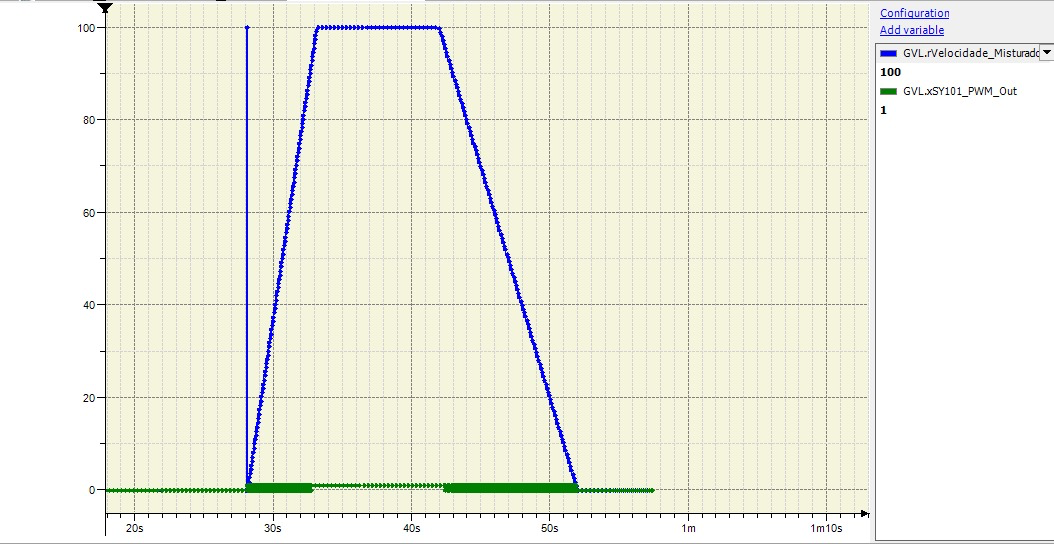
\includegraphics[width=0.6\textwidth]{imgs/pwm.png}
    \caption{Gráfico do PWM.}
\end{figure}

\subsection{Teste Área 1: Tanque RM-01}
Verificou-se o enchimento do tanque RM-01 a partir da atuação das válvulas de Gin e Vermouth, além do display de seu nível ao lado. Após as devidas proporções adicionadas, o misturador M-101 foi acionado. O ciclo de resfriamento da jaqueta foi verificado simulando os sensores de nível e temperatura. A válvula de refrigerante (FV-103) abriu corretamente ao iniciar a mistura e fechou imediatamente ao acionar o sensor de nível alto da jaqueta (LSH-102). 

\begin{figure}[H]
    \centering
    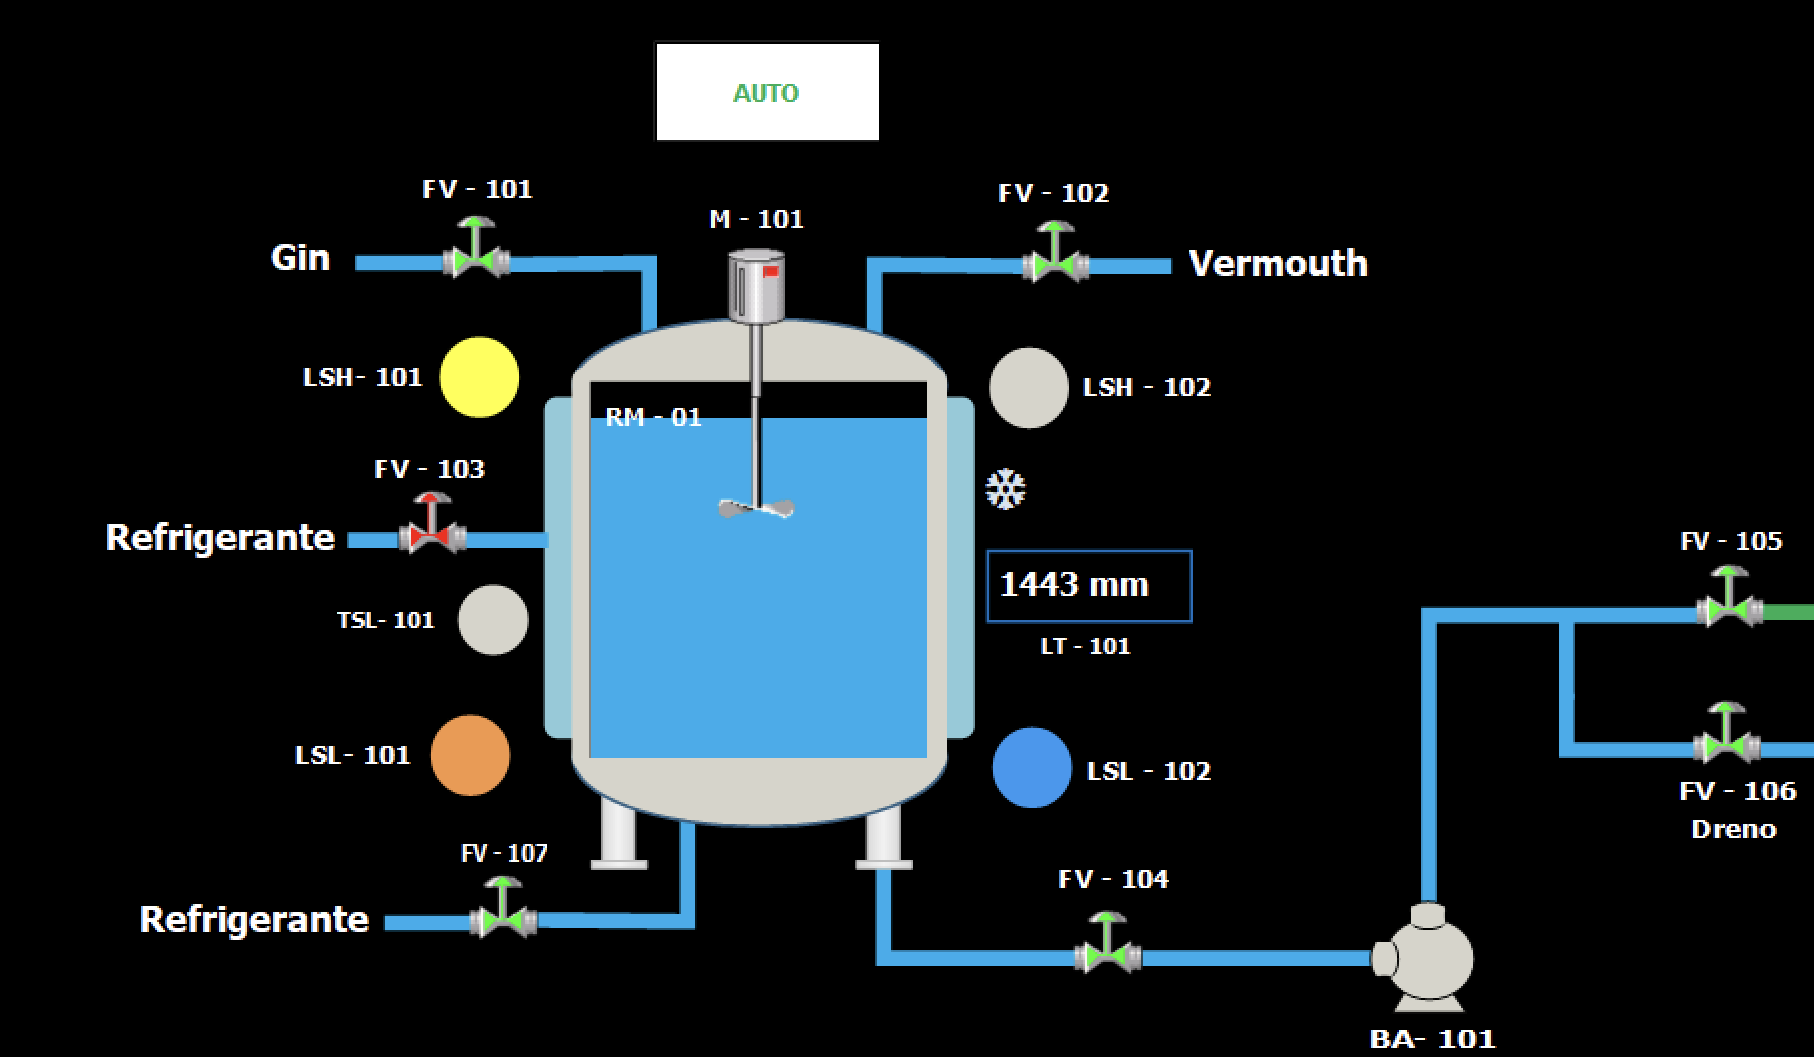
\includegraphics[width=0.6\textwidth]{imgs/rm_01.png}
    \caption{Tanque RM-01 com o misturador e a jaqueta em funcionamento.}
\end{figure}

\subsection{Teste de Envase}
Validou-se o funcionamento da Área 2: o TP-01 recebe o produto após a atuação das válvulas e da bomba BA-101 e, a partir da atuação da esteira, começa a encher os barris. A esteira só entra em operação quando o nível do Tanque de Produto supera 50\%, e desliga automaticamente quando o nível cai abaixo de 10\%, evitando oscilação do motor. Tudo isso com a correta implementação do sensor ZY-201, que identifica a presença do barril, e com a animação devida do bico injetor. Após o enchimento do barril, ele vai para o final da esteira, onde o sensor ZY-202 faz a contagem.

\begin{figure}[H]
    \centering
    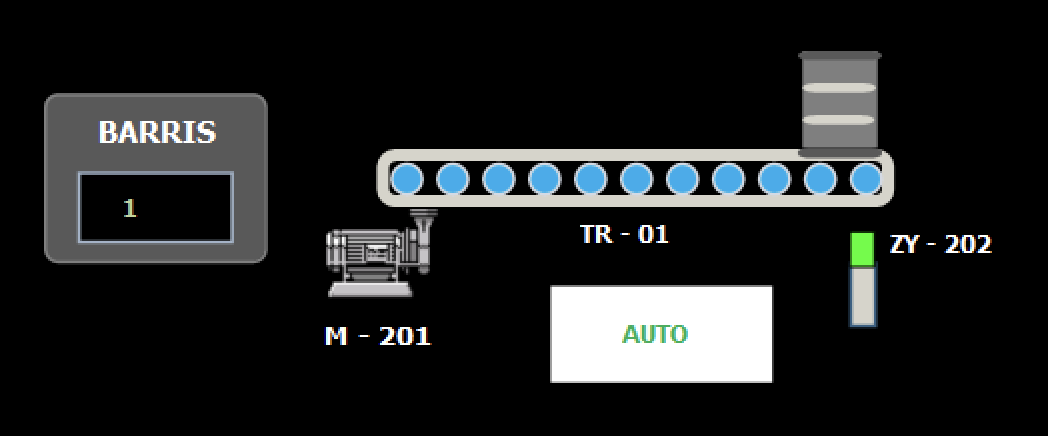
\includegraphics[width=0.6\textwidth]{imgs/contagem_barril.png}
    \caption{Contagem dos barris.}
\end{figure}

\subsection{Teste de Emergência}
Ao acionar o botão de Emergência durante a fase de mistura, o sistema interrompeu imediatamente o motor e as válvulas. Após o tempo de segurança (3s), a rota de descarte para o Tanque de Rejeitos foi aberta, validando a lógica de segurança implementada no SFC.
\begin{figure}[H]
    \centering
    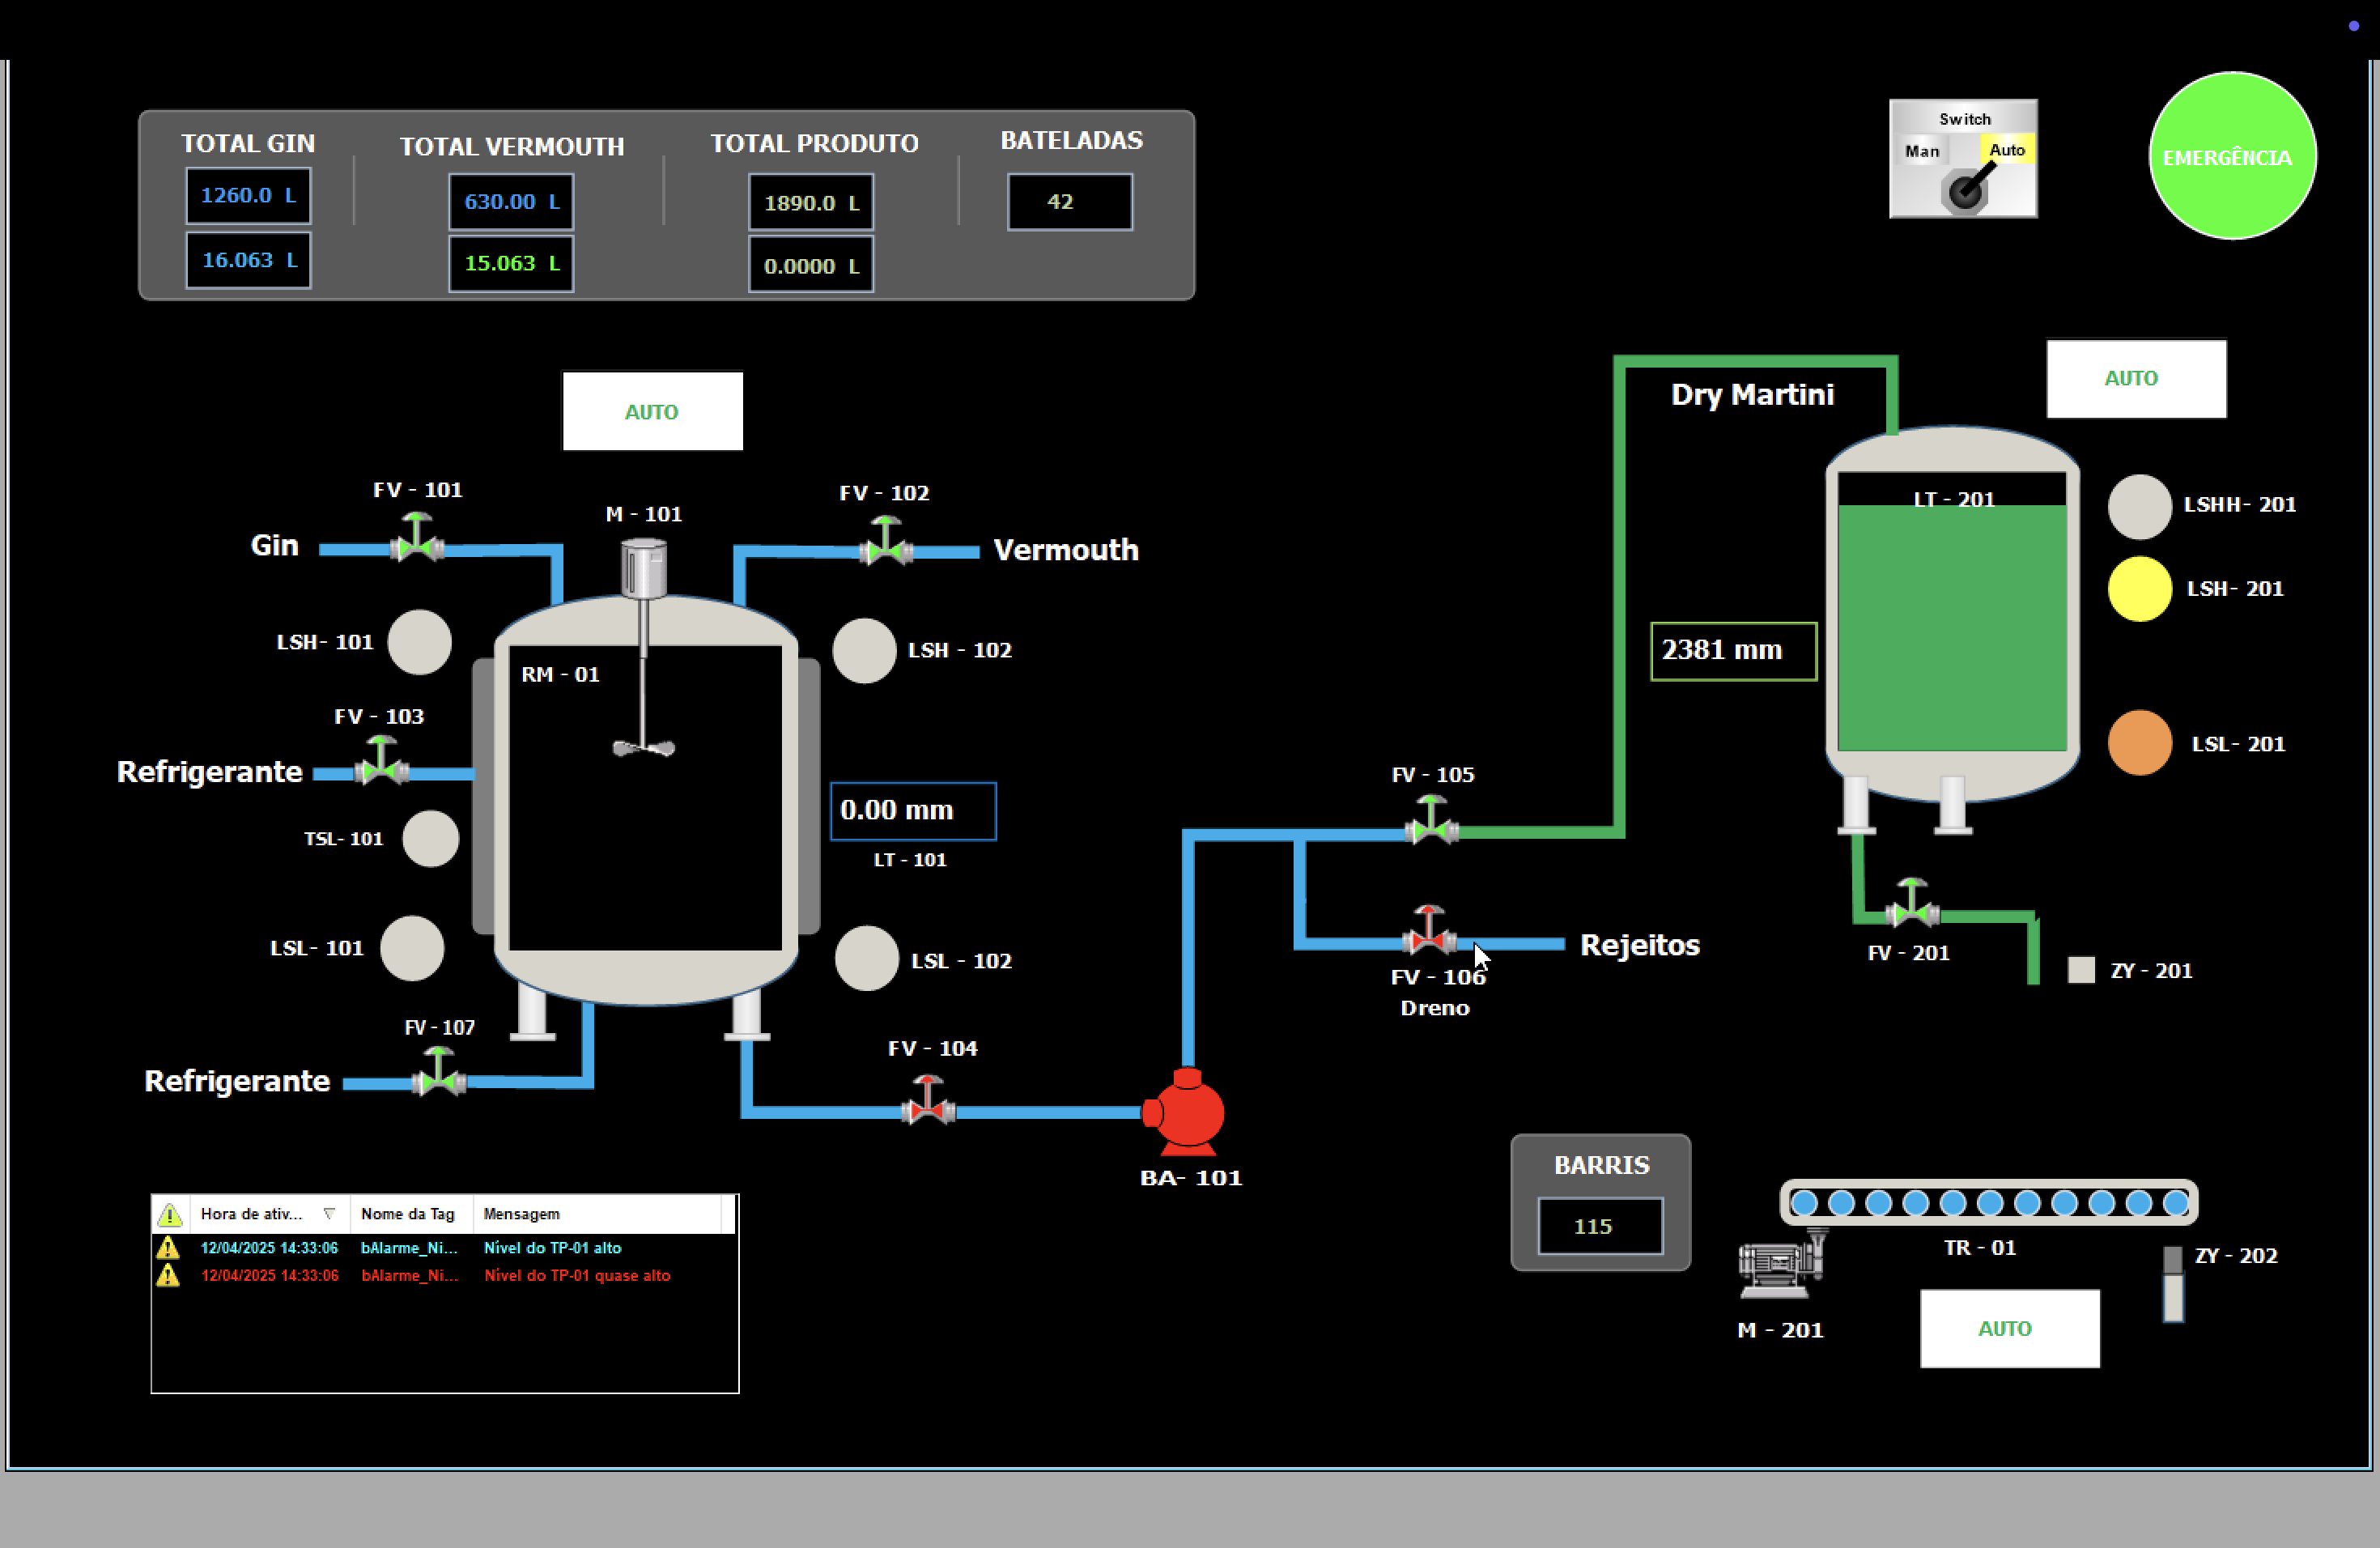
\includegraphics[width=0.6\textwidth]{imgs/emg_funcionando.png}
    \caption{Drenagem após apertar o botão de emergência.}
\end{figure}

\subsection{Validação dos Modos de Operação}
Alternou-se o sistema para o modo MANUAL na IHM. Verificou-se que a lógica sequencial (SFC) foi congelada e que o operador obteve controle individual sobre cada atuador (válvulas, bomba e motores), permitindo manobras de manutenção sem restrições de intertravamento lógico. Cada setor da tela do sinótico possui um identificador de qual modo está operando.

\subsection{Sensores, Totalizadores e Alarmes}
Todos os sensores discretos funcionam corretamente, identificando os respectivos níveis de seus tanques. Além disso, os totalizadores fazem a contagem correta da quantidade de cada produto, ciclo e barril, sendo mostrados em displays. Por fim, os alarmes mostram as mensagens correspondentes, podendo ser silenciados ou reconhecidos. 

\begin{figure}[H]
    \centering
    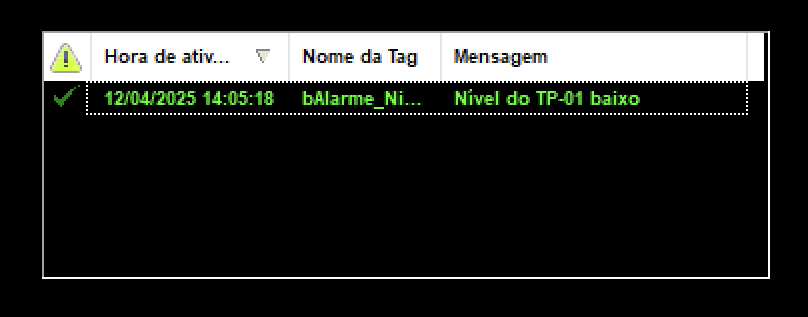
\includegraphics[width=0.5\textwidth]{imgs/reconhecimento_alarme.png}
    \caption{Reconhecimento de um alarme.}
\end{figure}

\begin{figure}[H]
    \centering
    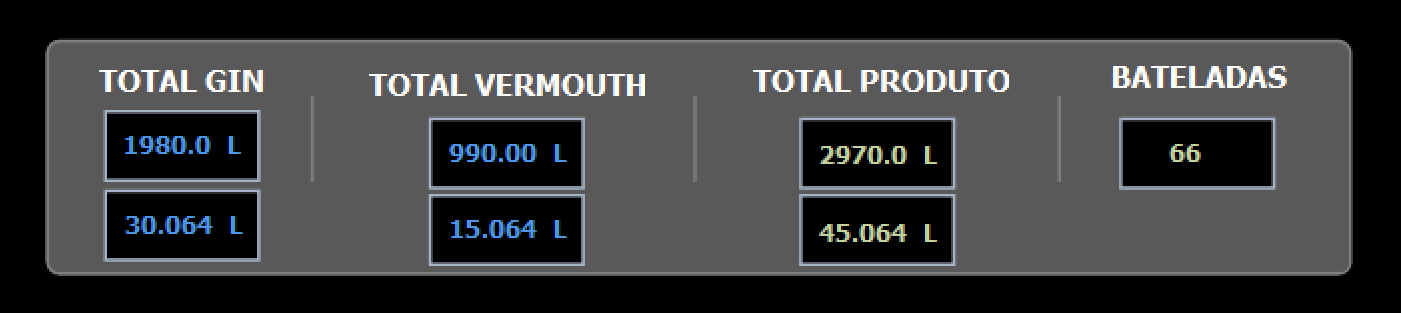
\includegraphics[width=0.5\textwidth]{imgs/totalizadores.png}
    \caption{Totalizadores mostrando a quantidade dos produtos e bateladas.}
\end{figure}
